% Standalone collection of ALL results, figures, tables, and statistics from
% the RA-L manuscript, labeled with the SAME numbering as the paper.
% Companion reference document. Not part of the submission.
\documentclass[11pt]{article}
\usepackage[margin=1in]{geometry}
\usepackage{graphicx}
\usepackage{amsmath,amssymb}
\usepackage{booktabs}
\usepackage{parskip}
\graphicspath{{figures/}}
\setlength{\parindent}{0pt}

\newcommand{\desc}[1]{\begin{quote}\small #1\end{quote}}

\begin{document}

\begin{center}
{\LARGE\bfseries Collected Results, Figures, Tables, and Statistics}\\[4pt]
{\large When Does Multimodal Diffusion Inverse Kinematics Help Soft Continuum
Arms---and Does It Survive Model Mismatch?}\\[4pt]
{\small Numbering matches the paper exactly. Every value traces to a committed
JSON in the repository root.}
\end{center}

\vspace{6pt}
\hrule
\vspace{10pt}

{\bf How the model works, once, up front.} The task is inverse kinematics for
a four-segment pneumatic continuum arm. Twelve chamber pressures determine a
three-dimensional tip position, so many distinct actuations reach the same
target and the inverse map is one-to-many. A regressor trained with mean
squared error fits the average of those valid answers, and the average of
distinct arm shapes is itself an invalid shape. The diffusion model avoids
this by never regressing the actuation directly. During training it corrupts
each dataset actuation with Gaussian noise at a random noise level and trains
a residual network, conditioned on the noise level and on the tip target
through feature-wise modulation, to predict the injected noise. Learning to
denoise at every noise level is equivalent to learning the gradient field of
the full conditional distribution over actuations, which preserves every
solution mode instead of their average. At query time the model starts from
32 independent Gaussian samples and deterministically refines each one
through 20 denoising steps, so different starting noise flows into different
solution modes and drawing samples is itself an enumeration of solutions.
Classifier-free guidance, trained by dropping the conditioning ten percent of
the time and applied at weight 1.5, sharpens accuracy while retaining
diversity. Each figure, table, and statistic below states how this mechanism
produces the result and what the result contributes to the paper.

\vspace{10pt}
\hrule

\section*{Table I. Core comparison on the PCC arm}

\begin{center}
\begin{tabular}{lcccc}
\toprule
 & Diffusion & grad-IK & MLP & MDN \\
\midrule
Tip err.\ best-of-$K$ (mm) & $0.44\pm0.03$ & $\mathbf{0.013}$ & $13.4\pm0.0$ & $17.3\pm0.2$ \\
Tip err.\ single sample (mm) & $\mathbf{1.69\pm0.15}$ & --- & $13.4\pm0.0$ & $83.6\pm2.7$ \\
Success @ 5 mm & $\mathbf{1.00}$ & $\mathbf{1.00}$ & $0.060$ & $0.027$ \\
Mode recall & $0.84\pm0.03$ & $\mathbf{0.85}$ & $0.00$ & $0.00$ \\
Diversity (curv.\ space) & $28.2\pm0.2$ & $\mathbf{29.0}$ & $0.0$ & $0.0$ \\
Obstacle success & $0.978\pm0.002$ & $\mathbf{0.980}$ & $0.040$ & $0.018$ \\
Query time (ms/target) & $38.6\pm4.9$ & $428$ & $\mathbf{0.013}$ & $0.022$ \\
\bottomrule
\end{tabular}

{\small (mean $\pm$ std over 3 training seeds, $K{=}32$ samples per target,
512 held-out targets for accuracy, 20 targets for mode recall, 200 obstacle
trials. grad-IK is one optimization run per target. A single-target diffusion
query costs about 84 ms.)}
\end{center}

\desc{The diffusion model samples 32 candidate actuations per target and the
best one lands within 0.44 mm of the target on average, with every target
solved at the 5 mm tolerance. Because the denoiser learned the whole
conditional distribution rather than its mean, its samples cover 84 percent
of the independently enumerated true solution modes, while the deterministic
MLP and the mixture density network recover none. The MLP fails because a
single output cannot represent multiple answers, and the MDN fails because
none of its mixture components is precise enough to pass the tolerance. The
classical optimizer grad-IK, given the true simulator to optimize through at
query time, matches or slightly exceeds the diffusion model on every task
metric, which shows that the learned model's real advantage is answering
from data alone at 5 to 11 times lower query cost with no simulator in the
loop. This table is the paper's foundation. It establishes the multimodality
advantage over learned baselines, and it honestly scopes the comparison
against classical optimization so that the transfer experiments later in the
paper test exactly the property, amortization, that makes the learned model
worth having.}

\section*{Fig. 1. Dataset-size ablation}

\begin{center}
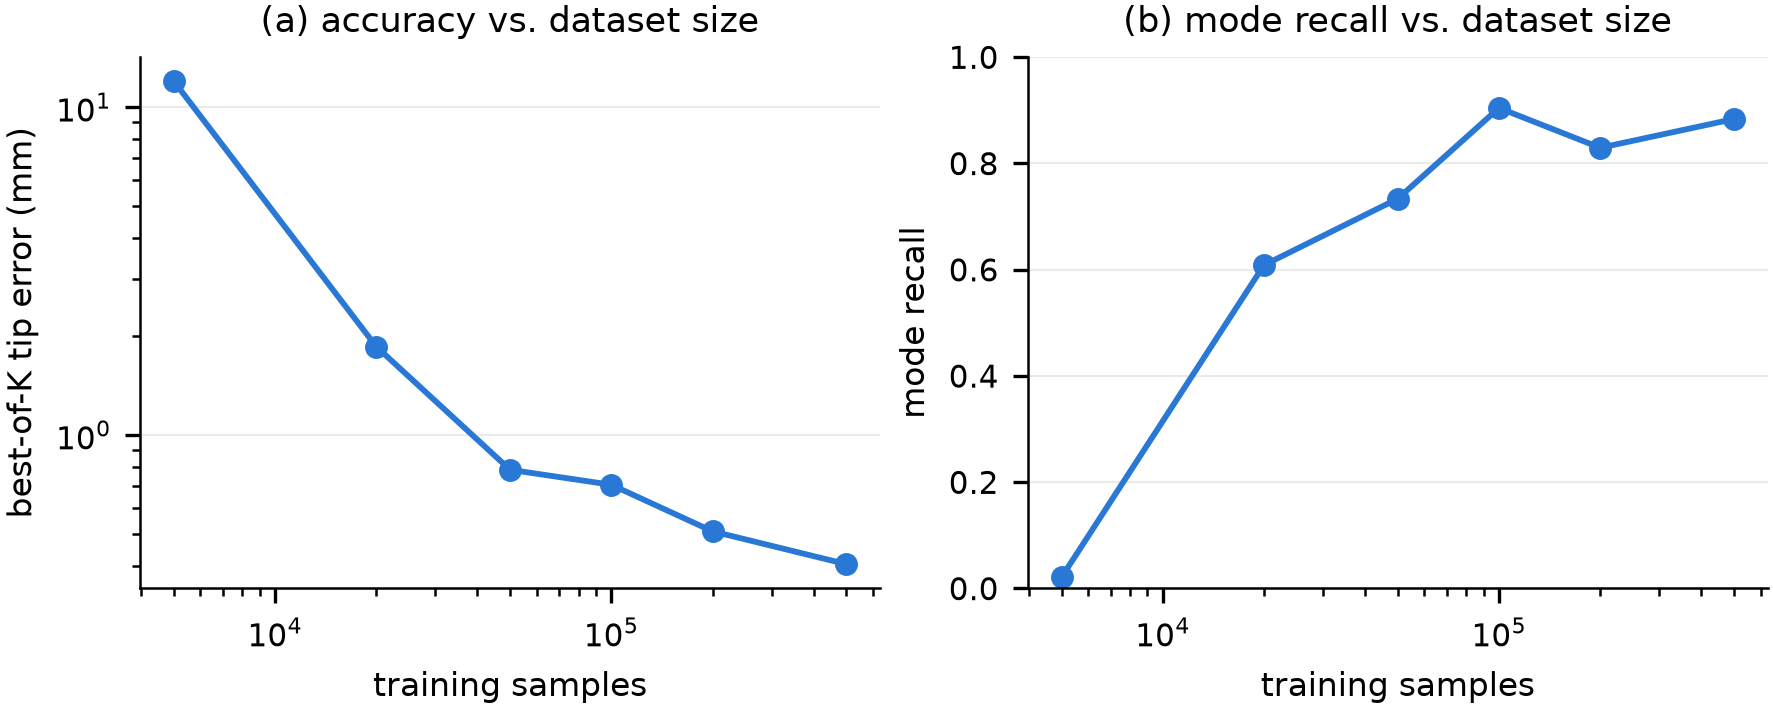
\includegraphics[width=0.85\linewidth]{fig_scaling.png}
\end{center}

\desc{The same diffusion architecture was retrained from scratch on datasets
from 5{,}000 up to 500{,}000 motor-babbling samples, single seed. Best-of-$K$
tip error and mode recall both saturate once the dataset reaches roughly
50{,}000 to 100{,}000 samples. The denoiser needs enough coverage of the
actuation space to learn the score field over all solution branches, and
beyond that coverage additional data adds nothing. The significance for the
paper is methodological. It shows the headline results are not starved for
data, so the baselines' failures cannot be blamed on dataset size, and it
tells a practitioner the data budget at which this approach becomes viable.}

\section*{Fig. 2. The advantage tracks redundancy}

\begin{center}
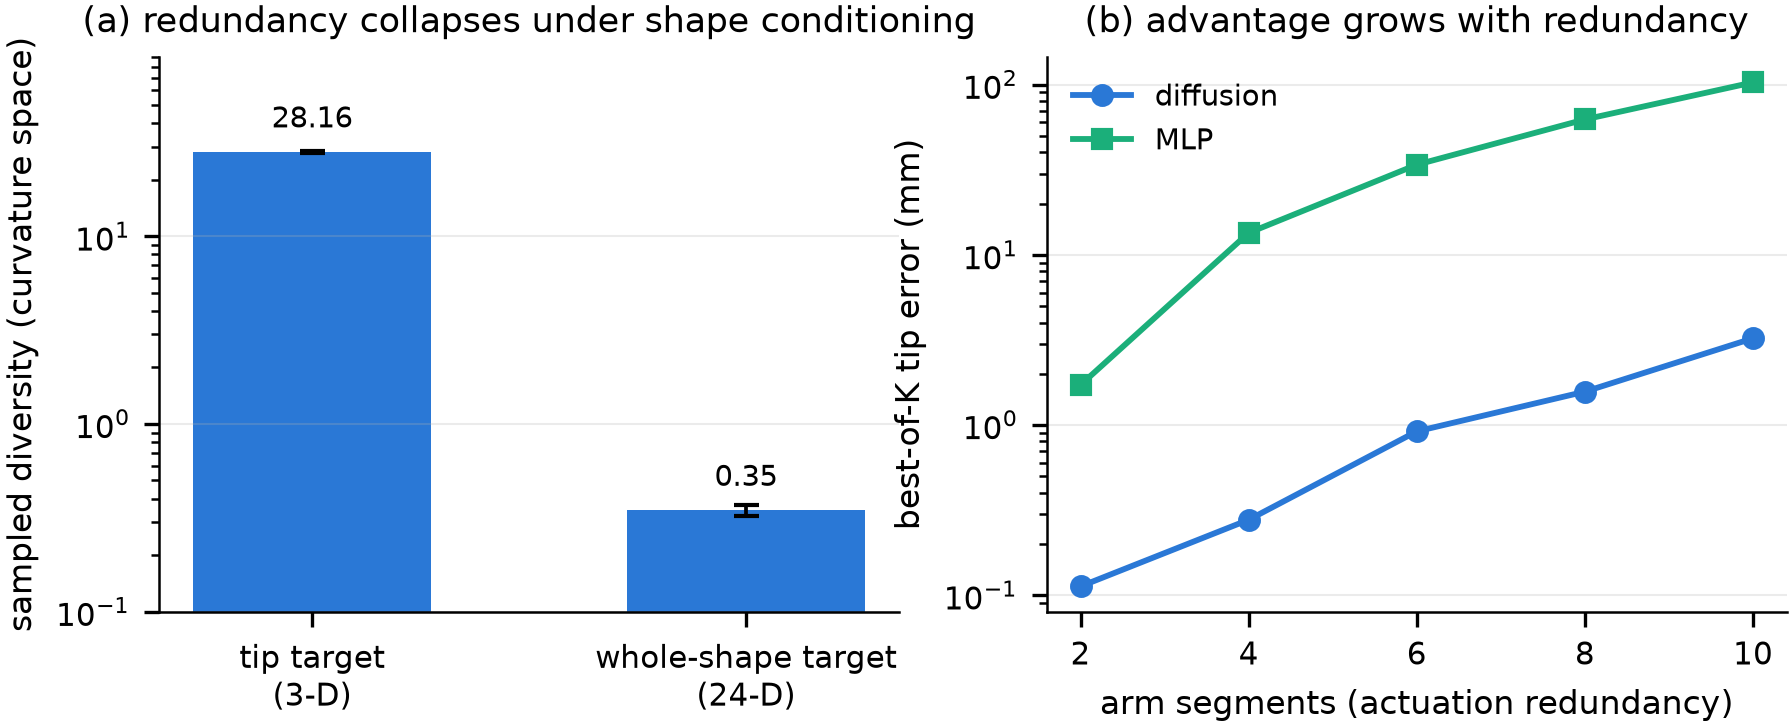
\includegraphics[width=0.95\linewidth]{fig_redundancy.png}
\end{center}

\desc{Panel (a) shows the shape-conditioning manipulation. Retraining the
same models with the 24-dimensional whole-arm shape as the conditioning
signal instead of the 3-dimensional tip removes almost all redundancy,
because specifying the whole shape pins down the actuation. The diffusion
model's sampled diversity collapses from $28.16\pm0.22$ to $0.346\pm0.022$,
a factor of about 80, and the MLP goes from about 30 times worse than
diffusion to only about 3 times worse, with both models at 100 percent
success. Panel (b) shows the morphology manipulation. Training fresh models on two,
four, six, eight, and ten segment versions of the arm adds or removes
actuation freedom, and the accuracy gap widens monotonically across all
five points, with the MLP at literal zero success from eight segments on
while diffusion holds at least 99.5 percent on the obstacle task.
The mechanism is that the denoiser represents whatever conditional
distribution the data presents. When conditioning removes the multimodality,
diffusion's samples concentrate onto the single answer and a deterministic
regressor is nearly as good. When morphology adds multimodality, mode
averaging hurts the regressor more while diffusion degrades gracefully.
These two manipulations are the paper's causal evidence that the advantage
in Table I is specifically redundancy resolution and not generic model
capacity.}

\section*{Table II. Recovery mechanisms at a glance (transfer domain)}

\begin{center}
\begin{tabular}{lccl}
\toprule
Mechanism & err (mm) & succ. & Cost / caveat \\
\midrule
none (top-1 candidate) & $161.5$ & $0\%$ & no target queries \\
best-of-32 selection & $130.4$ & $0\%$ & 32 queries/target \\
\; + diversity order & $-6.7$ at $m{=}8$ & $0\%$ & same queries, $p{\approx}0.002$ \\
guided sampling & $129.0$ & $0\%$ & 400 labels, suggestive \\
gain randomization & $140.6$ & $0\%$ & degrades source, no gain \\
fine-tune, $0\%$ mix & $\mathbf{67.1\pm0.9}$ & $\mathbf{10\%}$ & forgets source ($133$ mm) \\
fine-tune, $\geq 5\%$ mix & $\geq 133.8$ & $\leq 10\%$ & retains source, forfeits gain \\
\bottomrule
\end{tabular}

{\small (each row uses its own study's held-out target set of 15 to 45
targets. The 139.9 mm collapse figure quoted in the text corresponds to
best-of-8 selection.)}
\end{center}

\desc{The transfer experiment executes actuations sampled from the
PCC-trained diffusion model on a Cosserat-rod simulation of the same arm,
where accuracy collapses from $0.67\pm0.03$ mm to $139.9\pm1.8$ mm with zero
success on every seed. This table collects every mechanism the paper tests
for recovering that loss. Selection exploits the one thing a multimodal
model uniquely offers, many candidates to test in the target domain, but
even 32 target-domain evaluations per target leave the error at 26 times the
tolerance. Steering generation with a learned transfer-error regressor gives
a small held-out gain that does not survive multiple-comparison correction.
Randomizing the curvature gain during training recovers exactly nothing
because the mismatch between the simulators is directional rather than a
matter of scale. Only fine-tuning on target-domain data produces nonzero
success, and only in its most destructive form. The significance is the
paper's second headline. The learned inverse map is simulator specific, no
inference-time mechanism comes close to fixing it, and the one training-time
mechanism that works destroys the source domain, which motivates
parameter-level retention methods as the necessary next step.}

\section*{Fig. 3. Candidate selection under a query budget}

\begin{center}
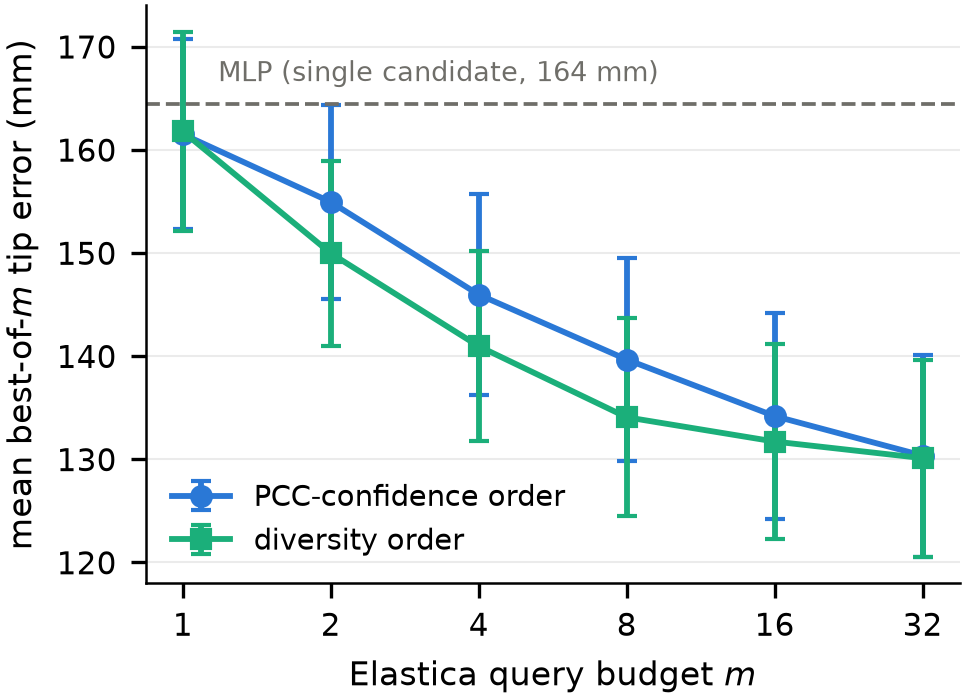
\includegraphics[width=0.85\linewidth]{fig_query_budget.png}
\end{center}

\desc{For 45 held-out targets the model samples 32 candidates each, and a
budget of $m$ expensive target-domain evaluations selects the best
candidate. Mean error falls from 161.5 mm at $m{=}1$ to 130.4 mm at
$m{=}32$, improving all 45 of 45 targets, yet success stays at zero at every
budget. The candidates are diverse because the denoiser spreads its samples
across the source domain's solution modes, and some of that spread happens
to land closer to the target domain's very different solution manifold,
which is why selection helps broadly but shallowly. A greedy
farthest-point ordering of the budget in curvature space beats spending the
budget in confidence order by 6.7 mm at $m{=}8$, the paper's strongest
statistical effect. The significance is a precise characterization of what
multimodality buys under model mismatch. It buys a real, broad, but bounded
improvement, and how the budget is spent matters more than how large it is,
while the transferred task itself remains unsolved.}

\section*{Table III. Fine-tuning and the retention--transfer cliff}

\begin{center}
\begin{tabular}{lcccc}
\toprule
PCC mix & PCC err (mm) & succ. & Elastica err (mm) & succ. \\
\midrule
none (baseline) & $0.44\pm0.03$ & $100\%$ & $151.1\pm2.5$ & $0\%$ \\
$0\%$  & $133.4\pm1.2$ & $0\%$ & $\mathbf{67.1\pm0.9}$ & $\mathbf{10\%}$ \\
$5\%$  & $30.7\pm0.6$ & $6\%$ & $133.8\pm3.1$ & $8\%$ \\
$10\%$ & $21.7\pm0.5$ & $17\%$ & $143.2\pm4.9$ & $8\%$ \\
$15\%$ & $16.7\pm0.2$ & $26\%$ & $146.0\pm3.4$ & $8\%$ \\
$20\%$ & $11.6\pm0.3$ & $51\%$ & $148.0\pm1.6$ & $10\%$ \\
$50\%$ & $3.0\pm0.4$ & $96\%$ & $152.3\pm0.4$ & $3\%$ \\
\bottomrule
\end{tabular}

{\small (mean $\pm$ std, 3 seeds. PCC columns use the 512-target evaluation,
Elastica columns use the same 20 held-out targets for every row including
the baseline.)}
\end{center}

\desc{The pretrained diffusion model is fine-tuned on 10{,}000
Elastica-simulated samples for 20 epochs at learning rate $3\times10^{-5}$,
with the stated fraction of each batch drawn from the original PCC data
through weighted sampling. Fine-tuning purely on target data rewrites the
denoiser's score field toward the target domain's solution distribution,
which produces the only nonzero transfer success in the paper, 67.1 mm and
10 percent, at the price of catastrophic forgetting of the source domain.
Mixing source data back in restores source accuracy smoothly and
monotonically down the left columns, but the transfer gain does not trade
off smoothly. At just 5 percent source data the transfer error has already
rebounded to 133.8 mm, forfeiting about 80 percent of the improvement over
the matched-target baseline of 151.1 mm, and it drifts only slowly after
that. The significance is that retention and transfer sit on a cliff rather
than a tradeoff curve, so no data-mixing ratio is a sweet spot, and the
paper's closing argument follows directly. Reshaping the model with small
amounts of target data requires protecting parameters, not rebalancing
batches.}

\section*{Fig. 4. The retention--transfer cliff}

\begin{center}
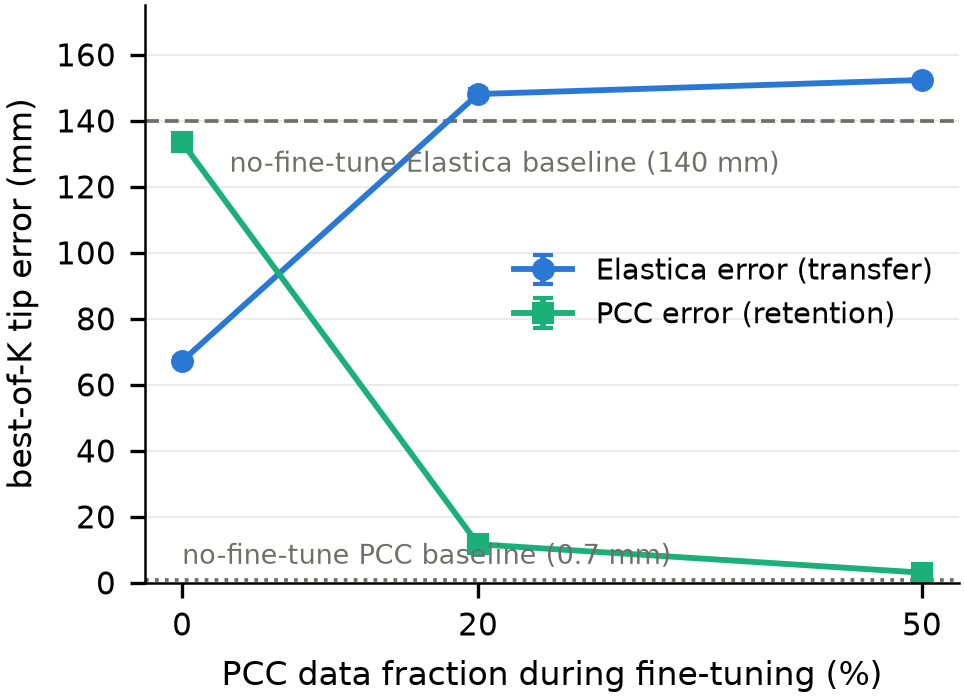
\includegraphics[width=0.85\linewidth]{fig_finetune_cliff.png}
\end{center}

\desc{This figure plots the two right columns of Table III against the
mixing ratio with three-seed error bars. The source-domain curve improves
smoothly and monotonically as source data is mixed back in, while the
target-domain curve loses nearly the entire fine-tuning gain by the first
grid point at 5 percent and stays flat afterward. The seed-to-seed standard
deviations of at most 4.9 mm show the cliff is not an unlucky training run.
Its significance is visual proof of the paper's final claim, the absence of
any data-mixing sweet spot, located by a sweep fine enough to place the
cliff's edge below 5 percent.}

\newpage
\section*{All remaining statistics, by paper section}

\subsection*{Section III, Setup}

\begin{itemize}
\item Ground-truth solution sets average $2.05$ modes per target, range 0 to
6, from a 2{,}000{,}000-sample sweep clustered with DBSCAN in curvature
space ($\varepsilon{=}12$, min\_samples${}=5$, match radius 15).
\item Settle-time convergence check, 8 random actuations. Tip shifts of 50
to 145 mm persist between integration horizons of 1.5, 3, 6, and 9 seconds.
\item Couple-gain calibration sweep over $5\times10^{-4}$ to
$5\times10^{-2}$. Mean tip discrepancy between simulators never falls below
about 150 mm while workspace radii stay similar (0.20 m versus 0.10 to 0.24
m).
\item Damping calibration sweep over constants 0.5 to 10. Changing the
damping moves the never-settled snapshot by up to 192 mm relative to the
default, yet mean tip discrepancy versus the PCC arm never falls below 149
mm at any value.
\item Transfer-collapse damping sensitivity. The same diffusion candidates
executed under Elastica at dampings 0.5, 2, and 8 give best-of-8 errors of
110, 120, and 145 mm with zero success at every value.
\end{itemize}

\desc{These numbers validate the evaluation machinery itself. Clustering in
curvature space matters because pressures contain a per-segment null space
that would corrupt distances. The settle check shows the target domain is a
fixed deterministic dynamic snapshot rather than an equilibrium, applied
identically everywhere, and the gain sweep shows the domain gap is
directional rather than a fixable unit mismatch. Together they certify that
the transfer collapse measured later is a property of the learned map, not
an artifact of calibration.}

\subsection*{Section IV, core experiments and ablations}

\begin{itemize}
\item Seed separation. On every task metric the worst diffusion seed beats
the best learned-baseline seed, for tip error 0.49 versus 13.33 mm, a gap
exceeding 400 times the across-seed standard deviation.
\item Guidance-weight ablation. Error 49.6 mm at weight 0, best 0.22 mm at
1.5, degrading to 3.1 mm at 3 and 13.2 mm at 4 with diversity collapsing
from 28.7 to 15.7. An inverted U with the operating point at its peak.
\item DDIM steps. Accuracy and recall saturate by about 20 steps, a 3 times
speedup over 50 steps at no measurable cost.
\item MDN fairness sweep over 4, 8, 16, 32 components. Best-of-$K$ error
improves only from 18.7 to 14.8 mm, never surpassing the plain MLP, and
mode recall is exactly zero at every setting.
\item MDN pathology. Training NLL decreases monotonically at every epoch, no
variance reaches its clamp floor, 7.8 of 8 components remain effective, yet
the best component mean per target carries 7.5 mm error against the 5 mm
tolerance, median component 9.2 mm.
\item Mode-enumeration sensitivity, 3 by 3 grid over $\varepsilon$ in
$\{10,12,14\}$ and match radius in $\{10,15,20\}$. Learned baselines recall
zero at all nine settings. Diffusion is higher at three settings, grad-IK at
five, one tie.
\item grad-IK compute ablation. At 100 iterations and 32 restarts it reaches
0.30 mm at 100 percent success in about 130 ms per target. Restart-RNG
variance across three seeds has standard deviation below 0.005 mm.
\end{itemize}

\desc{These statistics defend Table I against every fairness objection the
authors could construct. The seed-separation figure replaces formal testing
where three seeds would make it hollow. The two ablations show the
operating point was chosen at a validated optimum rather than tuned against
the baselines. The MDN analyses prove the multimodal baseline fails for a
substantive reason, imprecision, rather than a training pathology or an
under-tuned component count. The sensitivity grid shows the central
qualitative conclusion, multimodal methods recover modes and learned
regressors recover none, at every reasonable setting of the enumeration
hyperparameters. The grad-IK numbers quantify the honest cost comparison
that scopes the paper's claims.}

\subsection*{Section V, mechanism manipulations}

\begin{itemize}
\item Shape conditioning, 3 seeds. Diversity $28.16\pm0.22$ to
$0.346\pm0.022$, about 80 times. Accuracy gap shrinks from about 30 times
(13.4 versus 0.44 mm tip error) to about 3 times (0.49 versus 0.16 mm mean
per-backbone-point error), both models at 100 percent success.
\item Morphology, single seed per arm, five points. MLP error 1.7 mm at 75
percent success with two segments, then 13.5, 33.9, 62.5, and 103.2 mm with
success falling to literal zero from eight segments on. Diffusion 0.11,
0.28, 0.92, 1.57, and 3.23 mm with at least 99.8 percent success
throughout, always within the scaled 2 percent tolerance. Obstacle task
from eight segments on, at least 99.5 percent versus 0 percent.
\end{itemize}

\desc{These are the quantitative backbone of Fig. 2, showing both directions
of the causal manipulation with the numbers the figure plots. Their
significance is that the paper's central advantage rises and falls with the
amount of actuation redundancy and with nothing else that changed in the
experiments.}

\subsection*{Section VI, transfer and recovery}

\begin{itemize}
\item Transfer collapse, 3 seeds, 20 targets, $K{=}8$. Diffusion
$0.67\pm0.03$ mm at 100 percent on PCC falls to $139.9\pm1.8$ mm at 0
percent on Elastica. The MLP falls from 13.8 to $164.4$ mm.
\item Query budget, $n{=}45$. Error 161.5 (m=1), 154.9, 146.0, 139.7,
134.2, 130.4 mm (m=32). All 45 targets improve. Final gap to tolerance is
about 26 times.
\item Ordering comparison, paired within candidate sets. Diversity order
beats confidence order by 6.7 mm at $m{=}8$ ($t{=}3.34$,
$p{\approx}0.002$, 24 targets better versus 12) and 3.3 mm at $m{=}16$
($t{=}3.21$).
\item Predictor correlations at $n{=}45$, sized to detect $r{\geq}0.41$ at
80 percent power. Candidate diversity versus improvement $r{=}0.20$
($p{=}0.19$), Jacobian minimum singular value versus improvement $r{=}0.02$
($p{=}0.88$). A pilot effect at $n{=}20$ did not replicate.
\item Guided sampling, 15 held-out targets. Best-of-16 error 134.6 to 129.0
mm, paired improvement $5.6\pm2.5$ mm ($t{=}2.27$, $p{\approx}0.04$, 11 of
15 targets). Of the roughly six hypothesis tests in the paper only the
ordering result survives Bonferroni correction.
\item Combined 2 by 2 factorial, guidance by ordering. The mechanisms do not
stack. Guidance concentrates the candidate distribution while
diversity-ordering spreads selection.
\item Domain randomization, gain drawn uniformly from 15 to 35 per sample.
PCC accuracy degrades 0.44 to 2.18 mm and transfer is unchanged, 140.6 to
140.6 mm.
\item Fine-tune baseline matched to the fine-tuning target set. The base
models score $151.1\pm2.5$ mm at 0 percent on those 20 targets, making the
best fine-tuned result a 56 percent error reduction, and the 5 percent mix
forfeits about 80 percent of it.
\end{itemize}

\desc{This block is the complete statistical record of the paper's second
arc. The collapse numbers establish the problem on every seed. The budget
and ordering numbers quantify the ceiling of selection and identify how to
spend queries, with the ordering effect standing as the paper's only
correction-surviving significance. The null correlations, reported with
their power analysis, honestly retire a pilot hypothesis. The guidance,
factorial, and randomization results bound what steering and synthetic
variation can do. The matched baseline puts the fine-tuning gain and the
cliff on the same footing, closing the loop on the paper's final claim that
data mixing cannot smooth the retention-transfer tension.}

\subsection*{Efficiency summary}

\begin{itemize}
\item Diffusion 38.6 ms per target with 64 targets batched, about 84 ms for
a single-target query, 20 DDIM steps, CPU.
\item grad-IK 428 ms per target at the full budget, about 130 ms at the
reduced budget that still reaches 0.30 mm.
\item MLP 0.013 ms and MDN 0.022 ms per target, fastest by far and unable to
perform the task.
\end{itemize}

\desc{The timing numbers scope the amortization claim honestly, a 5 to 11
times advantage over the classical optimizer depending on batching, and they
matter because amortization without simulator access is precisely the
property the transfer experiments then show does not survive a change of
dynamics model.}

\end{document}
